\chapter{Упражнения по работе с пользовательскими функциями \unf}

Освоить работу с расчетными функциями \unf можно выполняя упражнения описанные в данном разделе и изучая устройство тестовых расчетных модулей. Упражнение демонстрируют некоторые подходы к использованию \unf. На основе этих подходов можно создать свои расчетные модули решающие специфические задачи пользователя. 

\section{Расчет PVT свойств}

Расчет физико химических свойств пластовых флюидов лежит в основе всех расчетов систем нефтедобычи. При решении прикладных задач редко возникает необходимость расчета PVT свойств непосредственно, однако понимание принципа их расчета, а особенно зависимости результатов расчета от исходных данных важно.
	
Цель упражнений по расчету PVT свойств:
\begin{itemize}	
	\item 	освоить принципы работы c пользовательскими функций \unf 
	\item 	изучить влияние исходных PVT данных на результаты расчета PVT свойств
	\item 	изучить влияние выбора PVT корреляций на результаты расчета PVT свойств
	\item 	изучить механизм калибровки PVT корреляций на результаты измерений
\end{itemize}
	 
	 
\subsection{Построение простых PVT зависимостей}

Для выполнения упражнения используйте файл "10.PVT.xlsx"

\begin{enumerate}
	\item Запустите файл с надстройкой \unf. Для того чтобы убедиться, что надстройка запущена откройте редактор VBE (Alt+F11). В дереве проектов должен отображаться файл надстройки \mintinline{vb.net}{UniflocVBA_7.xlam}, рис. \ref{ris:VBE_empty}.
	
	\begin{figure}[h!]
		\center{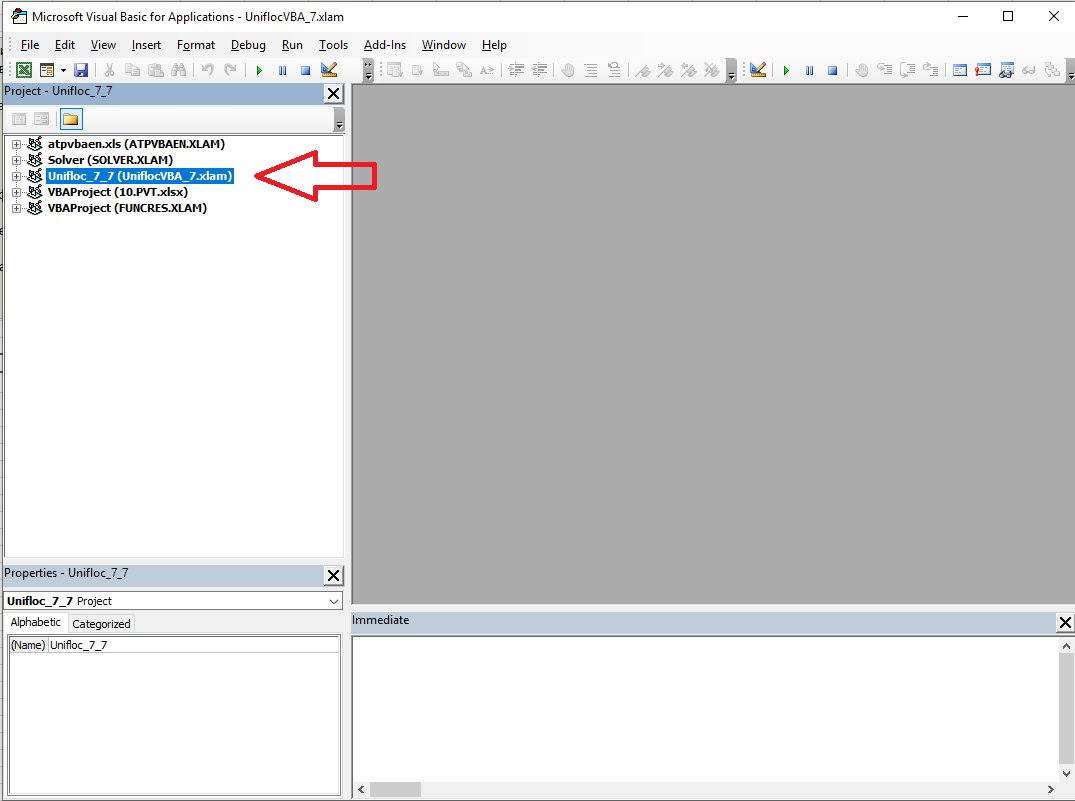
\includegraphics[width=0.5\linewidth]{VBE_empty}}
		\caption{Окно редактора VBE с загруженной надстройкой \unf}
		\label{ris:VBE_empty}
	\end{figure}

	\item Откройте файл с упражнением \texttt{10.PVT.xlsx} (смотри рис. \ref{ris:Ex10_1}).
	
	\begin{figure}[h!]
		\center{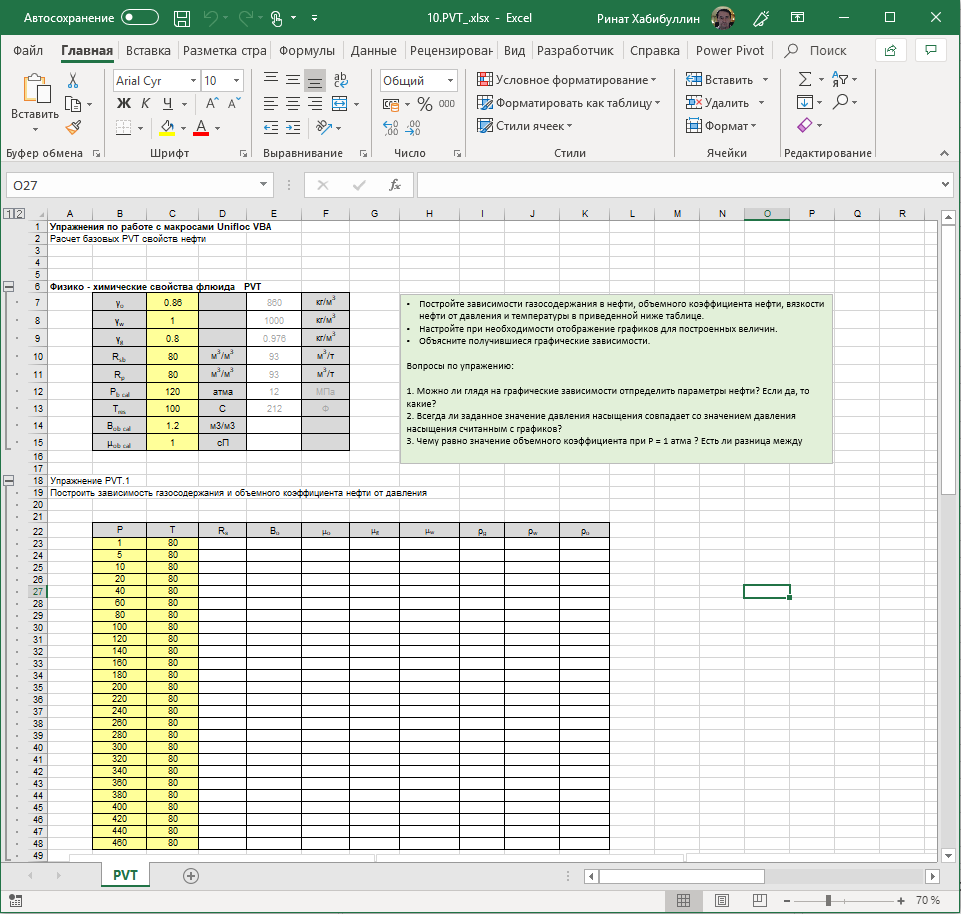
\includegraphics[width=0.5\linewidth]{Ex10_1}}
		\caption{Открытый файл с упражнением \texttt{10.PVT.xlsx}}
		\label{ris:Ex10_1}
	\end{figure}
	
	\item Для расчета первого элемента таблицы в ячейках D23:D48 - газосодержания в нефти при давлении 1 атм и температуре 80 °C - введите в ячейку D23 строку
	
	{ \small  \texttt{=PVT\_Rs\_m3m3(B23;C23;gamma\_gas\_;gamma\_oil\_; gamma\_wat\_; Rsb\_; Rp\_; Pb\_; Tres\_; Bob\_; muob\_)}}
	
	Обратите внимание -- при запущенной надстройке достаточно начать вводить в ячейку формулу, например ввести \texttt{=PVT} как Excel откроет выпадающий список с подсказкой, показывающий возможные варианты названий функций (смотри рис. \ref{ris:Ex10_2}). 
	
	В приведенной строке \texttt{B23;C23} - ссылки на соответствующие ячейки,  \texttt{gamma\_gas\_;gamma\_oil\_} - также ссылки на ячейки, которые предварительно были поименованы. 

	\begin{figure}[h!]
		\center{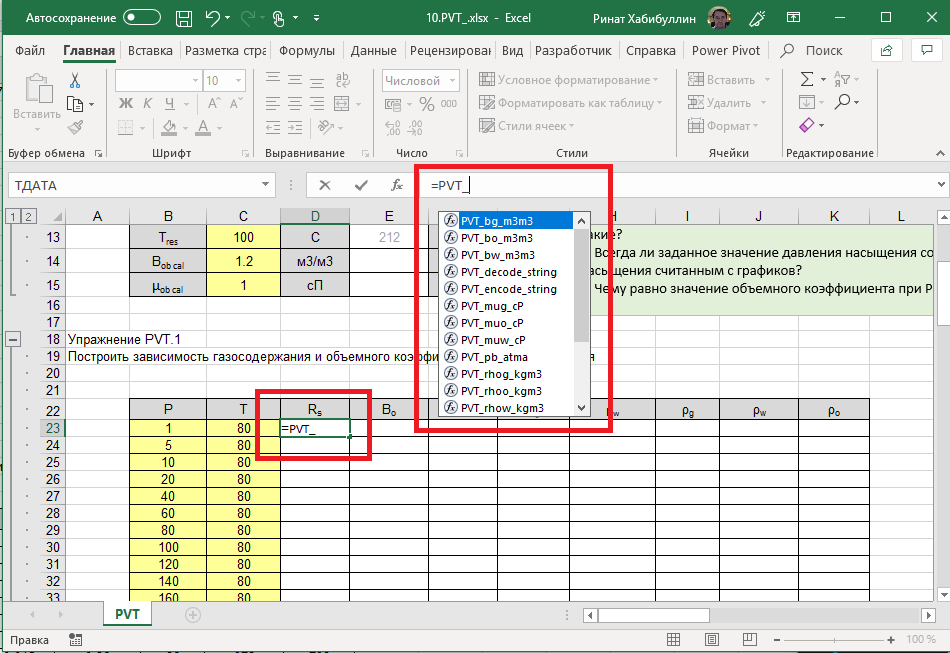
\includegraphics[width=0.5\linewidth]{Ex10_2}}
		\caption{Выпадающий список с подсказками названий функции}
		\label{ris:Ex10_2}
	\end{figure}

	Из выпадающего списка выберите функцию \texttt{=PVT\_Rs\_m3m3(} после чего нажмите кнопку $f_x$ "вставить функцию" слева от строки формул. Это вызовет окно задания параметров функции, в котором будут указаны все параметры, которые необходимо ввести. В этом окно можно ввести необходимые значения параметров или указать ссылки на соответствующие ячейки.

	\begin{figure}[h!]
		\center{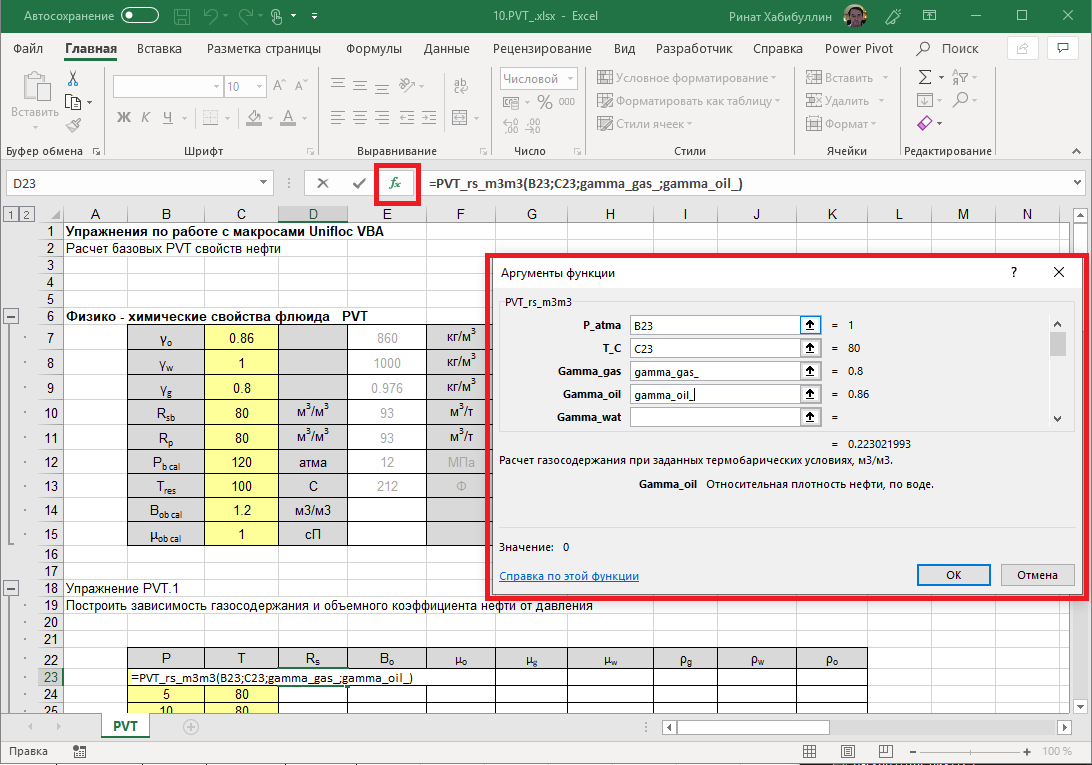
\includegraphics[width=0.5\linewidth]{Ex10_3}}
		\caption{Окно ввода аргументов функции}
		\label{ris:Ex10_3}
	\end{figure}

	\item После ввода всех параметров и нажатия кнопки ОК в ячейке должен отобразиться результат расчета. Воспользовавшись инструментом "Влияющие ячейки" на вкладке "Формулы" можно отследить на какие ячейки ссылается введенная формула
	\begin{figure}[h!]
		\center{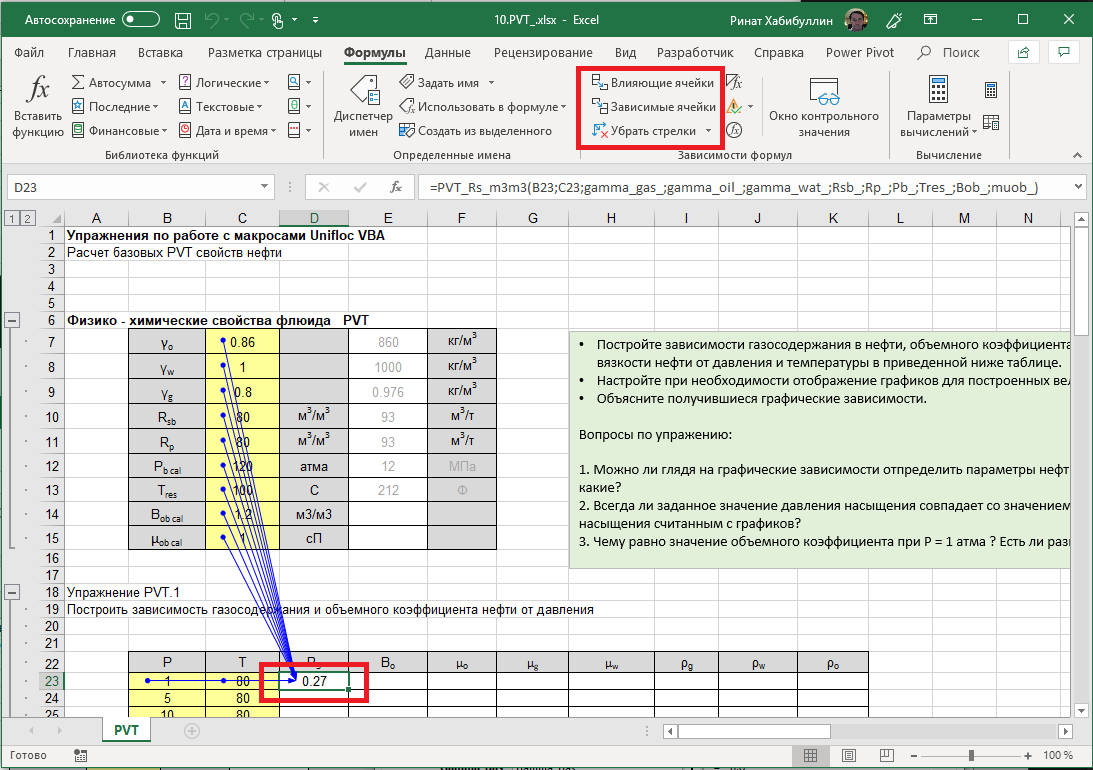
\includegraphics[width=0.5\linewidth]{Ex10_4}}
		\caption{Результат вызова пользовательской функции с отображение влияющих ячеек}
		\label{ris:Ex10_4}
	\end{figure}

	\item Аналогично заполните все ячейки таблицы  \texttt{D23:D48} вызовами функции \texttt{=PVT\_Rs\_m3m3()} с соответствующими параметрами. Это можно сделать "протянув" ранее введенную функцию в ячейке \texttt{D23}.
	
	Обратите внимание, что при "протягивании" поименованные ячейки оказываются закрепленными, а ссылки на значения давления и температуры съезжают вместе с протягиваемой ячейкой. Результат показан на рисунке \ref{ris:Ex10_5}
	\begin{figure}[h!]
		\center{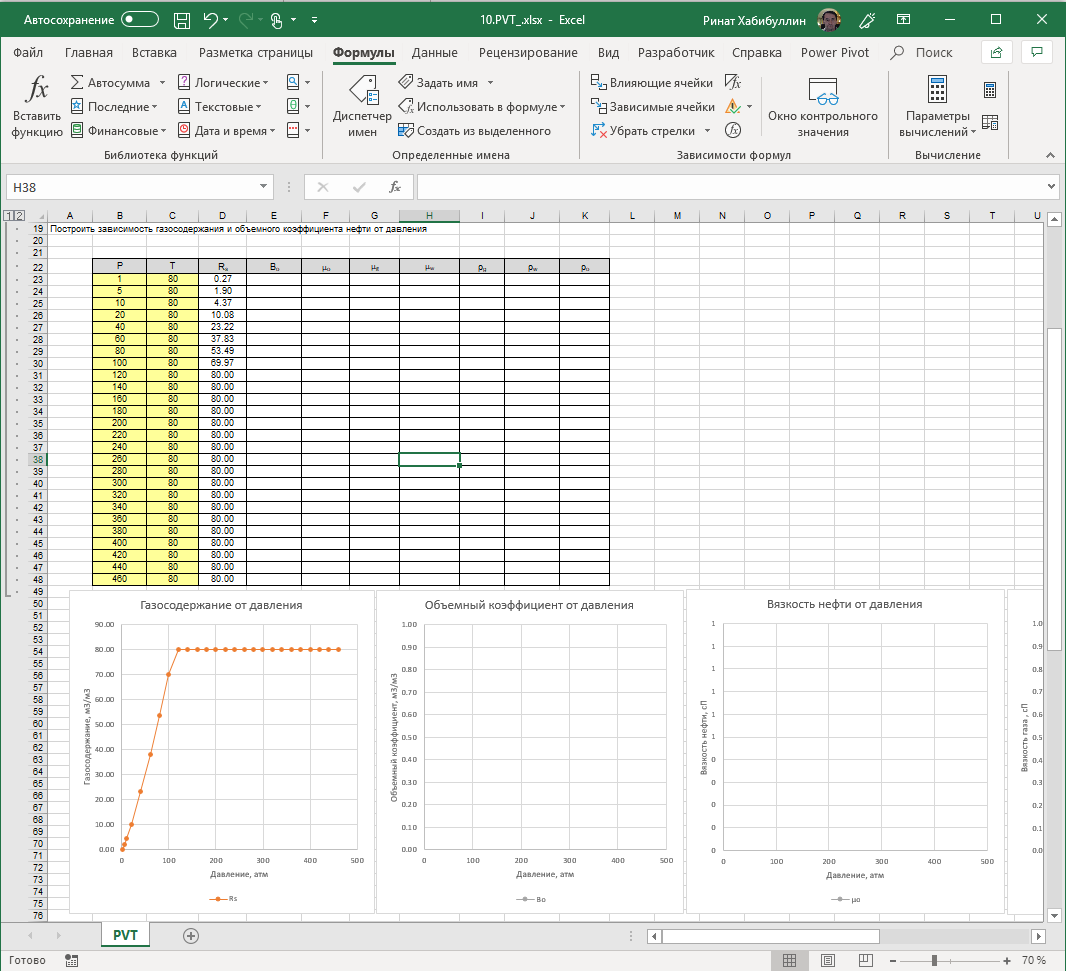
\includegraphics[width=0.5\linewidth]{Ex10_5}}
		\caption{Результат расчета зависимости газосодержания от давления}
		\label{ris:Ex10_5}
	\end{figure}

	\item По аналогии с зависимостью газосодержания от давления постройте графики зависимости других параметров от давления. Используйте следующие функции для проведения расчатов: 
	
	функция расчета объемного коэффициента нефти
	
	{ \small  \texttt{=PVT\_Bo\_m3m3(B23;C23;gamma\_gas\_;gamma\_oil\_;gamma\_wat\_; Rsb\_; Rp\_; Pb\_;Tres\_;Bob\_;muob\_)}}
	
	функция расчета вязкости нефти при заданных термобарических условиях
	
	{ \small  \texttt{=PVT\_Muo\_cP(B23;C23;gamma\_gas\_;gamma\_oil\_;gamma\_wat\_; Rsb\_; Rp\_; Pb\_;Tres\_;Bob\_;muob\_)}}
	
    функция расчета вязкости газа при заданных термобарических условиях
	
	{ \small  \texttt{=PVT\_Mug\_cP(B23;C23;gamma\_gas\_;gamma\_oil\_;gamma\_wat\_; Rsb\_; Rp\_; Pb\_;Pb\_;Bob\_;muob\_)}}
	
	функция расчета вязкости воды при заданных термобарических условиях
	
	{ \small  \texttt{=PVT\_Muw\_cP(B23;C23;gamma\_gas\_;gamma\_oil\_;gamma\_wat\_; Rsb\_; Rp\_; Pb\_;Tres\_;Bob\_;muob\_)}}
	
	функция расчета плотности газа при заданных термобарических условиях
	
	{ \small  \texttt{=PVT\_Rhog\_kgm3(B23;C23;gamma\_gas\_;gamma\_oil\_;gamma\_wat\_; Rsb\_; Rp\_; Pb\_;Tres\_;Bob\_;muob\_)}}
	
	функция расчета плотности воды при заданных термобарических условиях
	
	{ \small  \texttt{=PVT\_Rhow\_kgm3(B23;C23;gamma\_gas\_;gamma\_oil\_;gamma\_wat\_; Rsb\_; Rp\_; Pb\_;Tres\_;Bob\_;muob\_)}}
	
	функция расчета плотности нефти при заданных термобарических условиях
	
	{ \small  \texttt{=PVT\_Rhoo\_kgm3(B23;C23;gamma\_gas\_;gamma\_oil\_;gamma\_wat\_; Rsb\_; Rp\_; Pb\_;Tres\_;Bob\_;muob\_)}}
	
	Результаты приведены на рисунке \ref{ris:Ex10_6}
	
	\begin{figure}[h!]
		\center{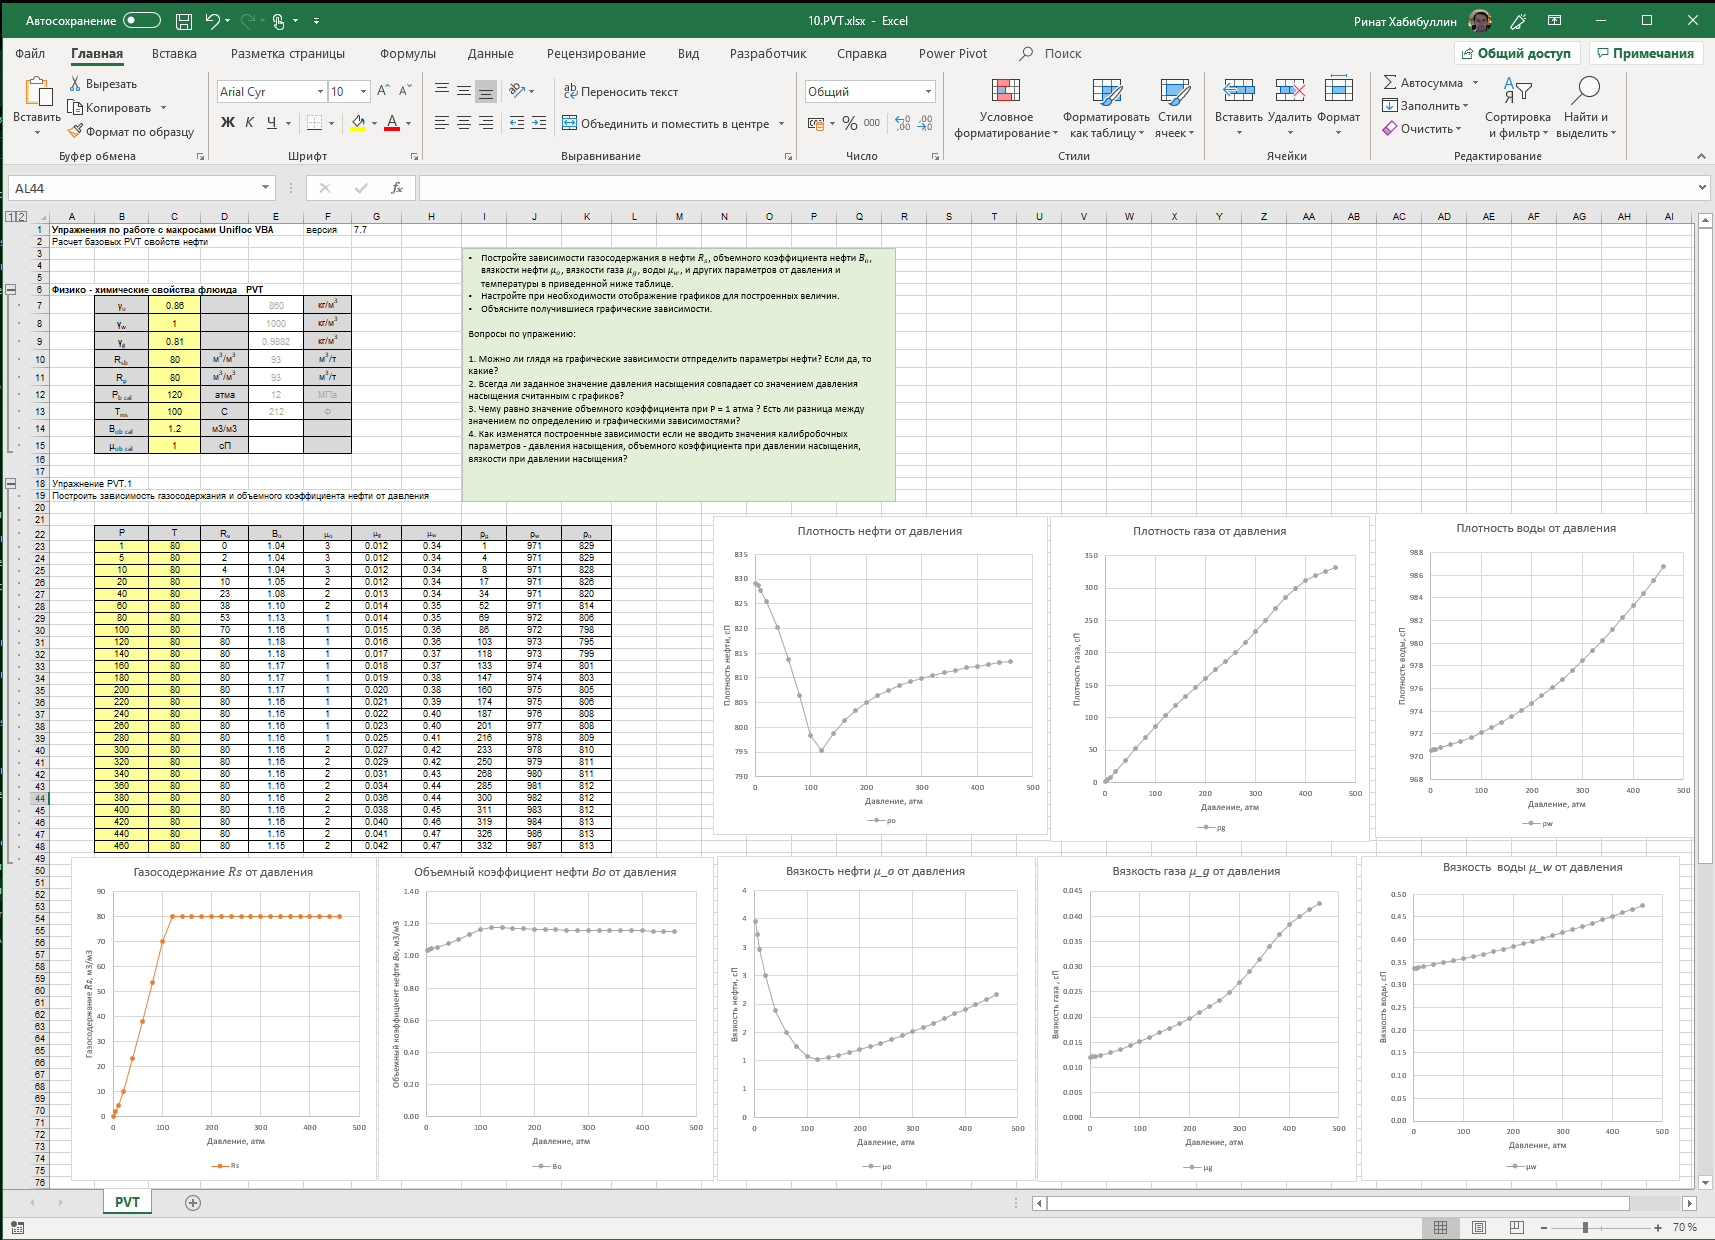
\includegraphics[width=1\linewidth]{Ex10_6}}
		\caption{Результат расчета зависимости свойств пластовых флюидов от давления}
		\label{ris:Ex10_6}
	\end{figure}
	
	\item Ответьте на вопросы по упражнению приведенные в рабочей книге.
	
	\begin{enumerate}
		\item Можно ли глядя на графические зависимости определить параметры нефти? Если да, то какие?
		\item Всегда ли заданное значение давления насыщения совпадает со значением давления насыщения считанным с графиков?
		\item Чему равно значение объемного коэффициента при Р = 1 атма? Есть ли разница между исходным значением и значением определенным по графическими зависимостями?
		\item Как изменятся построенные зависимости если не вводить значения калибровочных параметров - давления насыщения, объемного коэффициента при давлении насыщения, вязкости при давлении насыщения?
		
	\end{enumerate}
 
\end{enumerate}

\section{Набор расчетных модулей анализа скважины}
Пример использования алгоритмов \unf приведен в файле \texttt{UF7\_calc\_well.xlsm}.

Файл содержит набор расчетных модулей позволяющих провести анализ данных описывающих работу скважины с применением различных методов добычи.


\subsection{Расчетный модуль анализа и настройки PVT свойств}

